\documentclass[fleqn]{jbook}
\usepackage{physpub}

\begin{document}

\begin{question}{専攻 問題3}{}

% Definition of local macros
\def\fermiE{\varepsilon\ssub{F}}

一次元の自由電子系を考える。系の長さを$L$、温度を$T$、電子数を$N$と
する。一様な磁場$H$のもとで、ハミルトニアンは、
%
\[ {\cal H} = \sum_{i=1}^N\left(\frac{p_i^2}{2m}-\mu_iH\right) \]
%
と書かれるものとする。ただし、$m$は電子の質量、$p_i,\mu_i$はそれぞれ
$i$番目の電子の運動量とスピン磁気モーメントであり、$\mu_i$は
$\pm\muB$($\muB$はボーア磁子)の値だけをとる。また、$L$は十分
大きくて、電子状態に対する系の境界の影響は無視できるものとする。



\begin{subquestions}
\SubQuestion
  電子はボルツマン統計に従うものと仮定して次の問に答えよ。

  \begin{subsubquestions}
  \SubSubQuestion
    $H=0$の場合に、カノニカルアンサンブルにおける分配関数を求めよ。

  \SubSubQuestion
    それを用いて系の内部エネルギーを求めよ。

  \SubSubQuestion
    $H\neq 0$の場合は分配関数はどう書かれるか。

  \SubSubQuestion
    それを用いて比熱を求めよ。

  \SubSubQuestion
    系の磁化$M=\sum_i\Mean{\mu_i}/L$と$H$の間の関係を求めよ。
    ただし、$\Mean{}$は熱平均を表す。

  \SubSubQuestion
    帯磁率$\chi=\lim_{H\to 0}(M/H)$を求めよ。

  \end{subsubquestions}


\SubQuestion
  電子がフェルミ統計に従うことを考慮して次の問に答えよ。

  \begin{subsubquestions}
  \SubSubQuestion
    $T=0,\,H=0$における系の内部エネルギーをフェルミエネルギー
    $\fermiE$と$N$を用いて表せ。

  \SubSubQuestion
    $T=0$において、磁化$M$と磁場$H$の間の関係を求めよ。(結果は、
    $\muB H$と$2\fermiE $の大小関係によって異なることに注意せよ。)

  \SubSubQuestion
    帯磁率$\chi$を求めよ。{\bf 1}の(vi)で求めた$\chi$の$T=0$における
    振る舞いとの違いについて、物理的な理由をつけて説明せよ。

  \end{subsubquestions}
\end{subquestions}
\end{question}
\begin{answer}{専攻 問題3}{}

% Definition of local macros

\def\fermiE{\eps\ssub{F}}


\begin{subanswers}
\SubAnswer

  \begin{subsubanswers}
  \SubSubAnswer
    この電子系では電子同士の相互作用はないので、$N$個の電子は独立に
    振舞う。全体の分配関数$Z$は1電子系の分配関数$Z_1$によって
%
    \[ Z=Z_1^N \]
%
    と表される。$Z_1$ を求める。一次元の運動量空間は $h/L$ 単位に
    離散化されている。つまり、
%
    \[ p_n = \frac{h}{L}n \quad (n=0,\pm 1,\pm 2,\cdots) \]
%
    エネルギー$\eps$も離散値となり、$H=0$のとき、
%
    \begin{equation}
      \eps_n = \frac{p_n^2}{2m}%
                 = \frac{1}{2m}\Bigl(\frac{hn}{L}\Bigr)^2 \quad%
                   (n=0,\pm 1,\pm 2,\cdots) \eqname{1}
    \end{equation}
%
    となる。よって、
%
    \[ Z_1 = \sum_{n=-\infty}^{+\infty} e^{-\beta\eps_n}%
           = \frac{L}{h} \sum_{n=-\infty}^{+\infty} \frac{h}{L}%
             e^{-\frac{\beta}{2m}\left(\frac{hn}{L}\right)^2} \]
%
    $h/L\ll 1$なので、$\d{x}=h/L,\,x=nh/L$としてこの和を積分に変換する。
%
    \[ Z_1 = \frac{L}{h} \Iint{\d{x}} e^{-\frac{\beta}{2m}x^2}%
           = \frac{L}{h} \sqrt{\frac{2\pi m}{\beta}} \]

%
    よって全電子の分配関数は、同種粒子で区別できないことに注意して、
%
    \[ Z=\frac{1}{N!}\left(\frac{L}{h}\sqrt{\frac{2\pi m}{\beta}}\right)^N \]
%
    となる。

  \SubSubAnswer
    内部エネルギー$\Mean{E}$は分配関数より
%
    \[ \Mean{E} = -\Partial{}{\beta}\ln{Z}%
                = N \frac{\kB T}{2} \]
%
    と導かれる。


  \SubSubAnswer
    磁場のある場合のエネルギー$\eps$は次のようになる。
%
    \begin{equation}
      \eps_n = \frac{p^2}{2m} -\mu H = \frac{h^2}{2mL^2}n^2 - \mu H \quad (n=0,\pm 1,\pm 2,\cdots) \eqname{2}
    \end{equation}
%
    この時の$N$電子系、1電子系の分配関数をそれぞれ
    $Z'$、$Z_1'$ と表す。
%
    \[ Z_1' = \sum_\mu \sum_n e^{-\beta\eps_n}%
	    =  \sum_n e^{-\beta\frac{p_n^2}{2m}}%
               \sum_\mu e^{+\beta\mu H}%
	    = \frac{L}{h}\sqrt{\frac{2\pi m}{\beta}}%
              \left(e^{+\beta\muB H}+e^{-\beta\muB H}\right) \]
    \[ Z'   = \frac{1}{N!}Z_1^{\prime N}%
            = \frac{1}{N!}\left(\frac{L}{h}\sqrt{\frac{2\pi m}{\beta}}%
              \left(e^{+\beta\muB H}+e^{-\beta\muB H}\right)\right)^N
	    = \frac{1}{N!}\left(\frac{2L}{h}\sqrt{\frac{2\pi m}{\beta}}
              \cosh(\beta\muB H)\right)^N
\]
%
    となる。

  \SubSubAnswer
    内部エネルギー$\Mean{E}$は、
%
    \[ \Mean{E}  = -\Partial{}{\beta} \ln Z'%
	         =  N\frac{\kB T}{2}-\muB NH \tanh(\beta\muB H) \]
%
    よって比熱$C$は、
%
    \[ C  =  \Partial{\Mean{E}}{T}%
	  =  -\frac{1}{\kB T^2}\Partial{\Mean{E}}{\beta}%
	  =  \frac{1}{2}N \kB + N \kB \Bigl(\frac{\beta \muB H}{\cosh(\beta\muB H)}\Bigr)^2 \]


  \SubSubAnswer
    磁化$M$は一電子の磁気モーメントの熱平均$\Mean{\mu}$を用いて
%
    \[ M = \frac{1}{L} \sum_i\Mean{\mu_i} = \frac{N}{L}\Mean{\mu} \]
%
    と表される。この$\Mean{\mu}$は
%
    \[ \Mean{\mu} = \Partial{}{(\beta H)} \ln Z_1' %
	          = \muB \tanh{(\beta \muB  H)} \]
    よって、
%
    \[ M = \frac{N\muB}{L}\tanh{(\beta\muB  H)} \]
%
  \SubSubAnswer
    帯磁率$\chi$は
%
    \[ \chi = \lim_{H\to 0}\frac{M}{H}%
            = \Partial{M}{H}\Bigm|_{H=0}%
            = \frac{N}{L}\beta\muB ^2\frac{1}{\cosh^2(\beta\muB H)}\Bigm|_{H=0}%
            = \frac{N}{L}\frac{\muB ^2}{\kB T} \]

  \end{subsubanswers}


\SubAnswer

  \begin{subsubanswers}
  \SubSubAnswer
    電子のエネルギーは式\eqhref{1}で与えられており、これから
    逆に指定のエネルギー以下の状態の数 $n^{<}_{\eps}$が求まる。
    すなわち、
%
    \[ n^{<}_{\eps} = 2\sqrt{\frac{2mL^2}{h^2}} \sqrt{\eps} \]
%
    磁場が無い場合にはスピンは縮退していて、エネルギーの低い状態
    から一つの状態に2つの電子が入っていく。そのエネルギーの上端が
    $\fermiE$ である。よって電子の総数$N$は $2n^{<}_{\fermiE}$ で
    与えられることになり、
%
    \[ N=2n^{<}_{\fermiE}=4\sqrt{\frac{2mL^2}{h^2}} \sqrt{\fermiE} \]
%
    である。上の2式を整理して
%
    \[ n^{<}_{\eps} = \frac{N}{2\sqrt{\fermiE}} \sqrt{\eps} \]
%
    を得る。これから状態密度 $D(\eps)$ は、
%
    \[ D(\eps) = \Deriver{n^{<}_{\eps}}{\eps}%
          = \frac{N}{4\sqrt{\fermiE}} \frac{1}{\sqrt{\eps}} \]
%
    となる。

    さて、$T=0$において、fermionの分布関数$f(\eps)$は左下図の
    ようになっており、$\eps<\fermiE$の各状態に一様に電子が分布
    している。
    また状態密度 $D(\eps)$ は電子のスピンを考慮して縦軸に
    エネルギー、右軸に下スピンの状態密度、左軸に上スピンの状態密度を
    描くと右下図のようになっている。
%
    \begin{center}
      \mbox{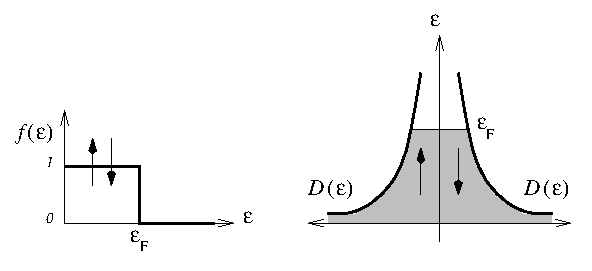
\includegraphics[clip]{1995phy3-1.eps}}
    \end{center}
%
    平均エネルギー $\Mean{E}$ を求める。上下スピン2種に電子がある
    ことに注意して$\eps$の平均値を求めると
%
    \[ \Mean{E} = 2\Dint{0}{\infty}{\d{\eps}} \eps f(\eps) D(\eps)%
                = 2\Dint{0}{\fermiE}{\d{\eps}} \eps D(\eps)%
	        = \frac{N}{2\sqrt{\fermiE}}%
                    \Dint{0}{\fermiE}{\d{\eps}}\sqrt{\eps}%
                = \frac{\fermiE N}{3} \]
%
    となる。

  \SubSubAnswer
    磁場のある場合の電子のエネルギー状態は式\eqhref{2}で与えられて
    おり、状態密度 $D_{\mu=\pm\muB}(\eps)$ を前問と同様に求めると
%
    \[ D_{\mu=\pm\muB}(\eps)=\frac{N}{4\sqrt{\fermiE}}\frac{1}{\sqrt{\eps\pm\muB H}} \]
%
    $\fermiE$は磁場の無い場合のフェルミエネルギーである。
    磁場のある場合のフェルミエネルギーを $\fermiE'$ とする。
    状態密度はスピンによって異なることになり、
    上スピン($\mu=+\muB$)の状態分布は $-\muB H<\eps<\fermiE'$
    であり、下スピン($\mu=-\muB$)の状態分布は $+\muB H<\eps<\fermiE'$
    である。\\
%
    $\fermiE' \ge \muB H$の場合には上下どちらのスピンの電子もあるが、
    $\fermiE'<\muB H$の場合には下スピンがなくなりすべて上スピンと
    なる。この様子を下図に示す。\\
%
    \parbox[t]{100mm}{
    上スピンの電子の個数を$N_+$、下スピンの電子の個数を$N_-$とする。
%
    \begin{eqnarray*}
      N_+ &=& \Dint{-\muB H}{\fermiE'}{\quad\d{\eps}}%
              \frac{N}{4\sqrt{\fermiE}}\frac{1}{\sqrt{\eps+\muB H}}%
           = \frac{N}{2\sqrt{\fermiE}}\sqrt{\fermiE'+\muB H}\\
      N_- &=& \Dint{+\muB H}{\fermiE'}{\quad\d{\eps}}%
              \frac{N}{4\sqrt{\fermiE}}\frac{1}{\sqrt{\eps-\muB H}}%
           = \frac{N}{2\sqrt{\fermiE}}\sqrt{\fermiE'-\muB H}\\
    \end{eqnarray*}
%
    磁化$M$は$\pm\muB$の磁気モーメントの平均なので
%
    \[ M = \frac{N_+}{L}\muB - \frac{N_-}{L}\muB %
         = \frac{\muB}{L}(N_+ - N_-) \]
%
    となる。

    $\fermiE'<\muB H$の場合には $N_-=0$となり、$N_+=N$となる。
    よって
%
    \[ M =  \frac{\muB N}{L} \hspace{10mm} (\fermiE'<\muB H) \]
%
    $\fermiE ' \ge \muB H$の場合には少々面倒で
%
    \[ N_+^2 - N_-^2 = \frac{\muB N^2}{2\fermiE} H \quad \mbox{より}\quad%
       N_+ - N_- =  \frac{\muB N}{2\fermiE} H \]
%
    が得られる。よって
%
    \[ M = \frac{\muB^2 N}{2L\fermiE} H = 
\frac{16mL\muB^2}{h^2N} H \hspace{10mm} (\fermiE ' \ge \muB H)\]
%
    となる。ところで、$\fermiE'=\muB H$の場合に$N_+=N$であることから
%
    \[ 2\fermiE = \muB H \]
%
    }\parbox[t]{50mm}{
    \begin{center}
      \mbox{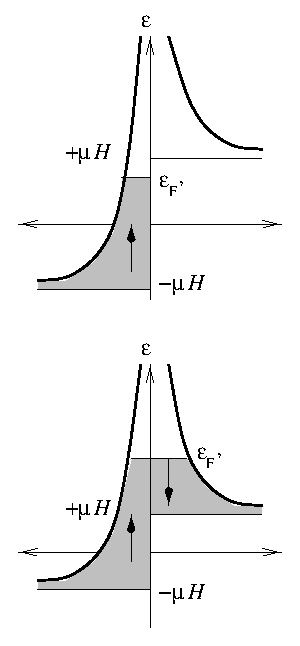
\includegraphics[clip]{1995phy3-2.eps}}
    \end{center}}\\
%
    の関係が得られる。すなわち先の $\fermiE'$と$\muB H$の
    大小の条件は  $2\fermiE$と$\muB H$の大小の条件に置き換えることが
    できる。


  \SubSubAnswer
    帯磁率$\chi$は
%
    \[ \chi = \lim_{H\to 0}\frac{M}{H} = \frac{16mL\muB^2}{h^2N} \]
%
    となり、一定の値を持つ。{\bf 1}(vi)でのボルツマン分布では
    $T\to 0$で発散していたのとは明らかに異なる。

    物理的には、ボルツマン統計は、エネルギー$E$の状態の起こる確率は、
    $e^{-\beta E}$に比例するとしているため、$T\to 0$では、ほとんど
    すべての粒子が最低エネルギー状態へ縮退してしまう。従って、
    $T\simeq 0$で磁場をかけると、わずかな磁場であってもほぼすべての
    電子が$E=-\muB H$の状態へ縮退し(スピンがすべて上向き)、磁化
    $M=N\muB/L$となる。従って、磁化率は$\infty$となる。しかし、
    このように一つの状態に$N$個の電子が詰まるという状態はPauliの
    排他律を考えれば起こるはずはなく、当然フェルミ統計に基づく結果
    とは、異なってくる。

  \end{subsubanswers}
\end{subanswers}

\end{answer}


\end{document}
